%%%%%%%%%%%%%%%%%%%%%%%%%%%%%%%%%%%%%%%%%%%%%%%%%%%%%%%%%%%%%%%%%%%%%%%%%%%%%%%%
%2345678901234567890123456789012345678901234567890123456789012345678901234567890
%        1         2         3         4         5         6         7         8

\documentclass[letterpaper, 10 pt, conference]{ieeeconf}  % Comment this line out
                                                          % if you need a4paper
%\documentclass[a4paper, 10pt, conference]{ieeeconf}      % Use this line for a4
                                                          % paper

\IEEEoverridecommandlockouts                              % This command is only
                                                          % needed if you want to
                                                          % use the \thanks command
\overrideIEEEmargins
% See the \addtolength command later in the file to balance the column lengths
% on the last page of the document



% The following packages can be found on http:\\www.ctan.org
\usepackage{graphics} % for pdf, bitmapped graphics files
\let\labelindent\relax
\usepackage{enumitem}
\usepackage{lipsum}
	

\usepackage{epsfig} % for postscript graphics files
\usepackage{mathptmx} % assumes new font selection scheme installed
\usepackage{times} % assumes new font selection scheme installed
\usepackage{amsmath} % assumes amsmath package installed
\usepackage{amssymb}  % assumes amsmath package installed
\usepackage{cite}  % for easy citing outputs
\usepackage{color}
\usepackage{microtype}
\usepackage{graphicx}
\long\def\dv#1{\textcolor{red}{**[DV] #1**}}
\long\def\zt#1{\textcolor{cyan}{**[ZT] #1**}}

\usepackage[caption=false,font=footnotesize]{subfig}
\usepackage{algorithmic}
\usepackage{algorithm}
\pdfminorversion=4
\usepackage{epstopdf}
%\title{Uncertainty-based Human-Aware Navigation}

\title{Incorporating Perception Uncertainty in Human-Aware Navigation: A Comparative Study}

\author{Zeynab Talebpour$^{1}$ \and Deepak Viswanathan$^{2}$ \and Rodrigo Ventura$^{3}$ \and Alcherio Martinoli$^{4}$ \and Gwenn Englebienne$^{5}$  % <-this % stops a space
\thanks{$^{1,4}$Distributed Intelligent Systems and Algorithms Laboratory,
School of Architecture, Civil and Environmental Engineering,
 \'Ecole Polytechnique F\'ed\'erale de Lausanne 
        {\tt\small \{zeynab.talebpour, alcherio.martinoli\}@epfl.ch}}% <-this % stops a space
\thanks{$^{2}$Deepak Viswanathan, Department of Informatics, University of Amsterdam
        {\tt\small D.geethaviswanathan@uva.nl}}%
\thanks{$^{3}$Rodrigo Ventura, Institute for Systems and Robotics, Instituto Superior T\'ecnico, Universidade de Lisboa, Portugal
        {\tt\small  rodrigo.ventura@isr.ist.utl.pt}}%
\thanks{$^{5}$Gwenn Englebienne, Human Media Interaction Laboratory, University of Twente, Netherlands
        {\tt\small g.englebienne@utwente.nl}}%
%\thanks{This research was supported by the European MOnarCH project FP7-ICT-9-2011-601033.}%
}

\begin{document}



\maketitle
\thispagestyle{empty}
\pagestyle{empty}


%%%%%%%%%%%%%%%%%%%%%%%%%%%%%%%%%%%%%%%%%%%%%%%%%%%%%%%%%%%%%%%%%%%%%%%%%%%%%%%%
\begin{abstract}
%In this work, we present a novel approach to human-aware navigation based on the fast marching method, by probabilistically modeling the uncertainty in on-board perception components of a social robotic system and investigating its effect on the overall social navigation performance. We have extended the model of the social costmap around a person to consider this new uncertainty factor which plays an important role in situations with noisy perception. Real robot experiments have been carried out to show the effectiveness of our approach in realistic scenarios with noisy perception involving a single dynamic human. Results show how our approach has been able to achieve trajectories which are more socially-aware compared to the basic navigation approach, and the human-aware navigation approach which relies solely on perfect perception.
In this work, we present a novel approach to human-aware navigation based on the fast marching method, by probabilistically modeling the uncertainty of perception for a social robotic system and investigating its effect on the overall social navigation performance. We have extended the model of the social costmap around a person to consider this new uncertainty factor which plays an important role in situations with noisy perception. Additionally, a variation of the Dynamic Window Approach, which takes social costs into account, had been considered for navigation to discard or penalize velocity candidates that lead to unnatural and uncomfortable moments in the vicinity of humans. 
Real robot experiments have been carried out to show the effectiveness of our approach in realistic scenarios with noisy perception involving a single dynamic human. Results show how our approach has been able to achieve trajectories which are more socially-aware compared to the basic navigation approach, and the human-aware navigation approach which relies solely on perfect perception.

\end{abstract}


%%%%%%%%%%%%%%%%%%%%%%%%%%%%%%%%%%%%%%%%%%%%%%%%%%%%%%%%%%%%%%%%%%%%%%%%%%%%%%%%
\section{Introduction}


Robots will progressively become part of the work spaces and habitats of humans.
Despite where they are located, in home environments or hospitals as assistants, in factories as co-workers or as guides in supermarkets, a key behavior which they all share is navigation.
Robots have to navigate in environments shared with humans and the quality of their movement strongly influences  how their intelligence is perceived~\cite{Althaus2004}. Consequently, new methods for robot navigation in the presence of humans are being studied extensively. Kruse et al.~\cite{Kruse2013} present a thorough survey of such methods where they identify comfort, naturalness and scalability as the three key issues addressed by the existing human-aware robot navigation methods so far. %(last 2 sentences taken from  RV's paper)
%Hence socially-aware navigation which pays special consideration to people 

Presence of humans in an environment should be properly perceived by a robot as a requirement for a socially-aware path planner that takes into consideration individual humans and possible social interactions taking place in the environment. This information can be obtained by an external source such as an overhead camera or can be attained using on-board sensors of the robot. while there are advantages and disadvantage to both cases, on-board perception allows for a fully autonomous and independent robot that relies only on itself for taking decisions about the world. Moreover, there are environments which do not permit the use of external infrastructures required for providing the requisite perception, due to reasons such as privacy or security issues or etc. Therefore, providing the required perception for human-aware navigation with on-board sensors is a desirable characteristic for a robot which helps integration of such systems into real-world environments.  


However, perception will never be perfect and is affected by various elements such as the movement of the robot, movement of the person, complexity of the environment in terms of occlusions, etc. Unlike other works which choose to ignore this very important aspect of the uncertainty in perception, we propose a model which computes the uncertainty of the location and orientation of the people in an environment. We aim to study, how this factor should influences the social costs used by the path planner and how taking this into account the resulting trajectories will be improved in terms of social acceptability.

One important concept which is used in numerous studies~\cite{Mumm2011,Takayama2009,Walters2011,ferrer2013robot} in this area is virtual space around a person that is mutually respected by other humans, called \textit{proxemics}~\cite{Hall1969}.
Based on this concept, depending on the relationship and the interaction that exists between humans, people choose different social distances relating to intimate, personal, social or public contexts.
Changes in the expected distance may indicate dislike if it is too large or cause discomfort if it is too small.



As stated in~\cite{gomez2013social}, recent work in the human-robot interaction domain can be divided in three categories of 1) human-robot proxemics, 2) human-aware planning and navigation, and 3) robot-to-human approaching and behaving. In this work we focus mostly on the second category using the concepts from human-robot proxemics. %Human-aware path planning has been an area of interest particularly in the recent years. 

In this research we are introduce a social path planning approach based on the fast marching method (FMM)~\cite{sethian1999fast} which has been proven to be successful in real domestic spaces \cite{ventura2015}. However, we add a social component to the aforementioned method by augmenting it with social costmaps \textemdash based on proxemics principles~\cite{kirby2009companion}\textemdash~around individual people which correspond to speedmaps for the FMM method. There have previously been a number of research papers which have address social path planning~\cite{gomez2014fast,gomez2013social} using FMM. 

The work of ~\cite{gomez2014fast} a theoretical framework for introduced sub-problems of social path planning is presented and an extended mode for engaging groups of people is proposed by using a special version of fast marching square planning method~\cite{valero2013fast}. Nonetheless, the information about humans are considered to be given and noiseless, while only simulations have been used to show the effectiveness of the proposed method for static people. We are interested in investigating the same problem in real-world scenarios with the challenges that exist therein. Particularly, in the case of moving people, while the perception is obtained only by the use of on-board resources of the robot and is consequently subject to different levels of uncertainty. 
%We believe that uncertainty of perception in social robotics is an important topic which to our knowledge is very little explored.
We believe that uncertainty of perception in social robotics, is an important topic which to our knowledge, has not been the subject of notable explorations. There is a dedicated chapter in \cite{correa2014uncertainty} on local planning with uncertainty, however this is not considered in a social context. The sources of uncertainty in~\cite{correa2014uncertainty} are the position of the robot and the obstacles, and the partially known motion of moving obstacles.


The remainder of this article is organized as follows. In section~\ref{sec:background} we introduce the background for this work. In section~\ref{sec:results}, we show the results of real robot experiments and finally, section~\ref{sec:conclusion} concludes this work.

%\paragraph{Story}  - Quantify uncertainity in perception. Use this for generating cost maps adaptively. FMM creates plans using this uncertainity model.





% \paragraph{Motivation and approach} - Perception will never be perfect. Unlike other works which choose to ignore this very important aspect of the uncertainty in perception, we propose a model which computes the uncertainty of the location and orientation of multiple people in an environment. We use this model to make informed choices about the cost function for navigation which is then used by a state of the art navigation model using FMM. We dynamically replan based on the perception information available. The key idea is that in cases where the perception is unreliable, we need to make sure that the robot navigates prioritizing safety over social norms.

% paragraph{Note} Active perception is also important. The robot movement causes uncertainty which can be actively reduced by taking paths which improve the perception information.

\section{Background}
\label{sec:background}
background
\section{perception model}
\label{sec: perception model}
%The uncertainity based human-aware navigation system, is comprised of several key components, i.e., probabilistic perception, social path planning and navigation. In this section we will briefly explain each of the parts of our model.


Presence of humans in an environment should be properly perceived by a robot as a requirement for a socially-aware path planner that takes into consideration individual humans and possible social interactions taking place in the environment. This information can be obtained by an external source such as an overhead camera or can be attained using on-board sensors of the robot. Different perception sources for person detection and tracking, have different levels of uncertainty and accuracy in their detections, and are affected by various elements such as the movement of the robot, movement of the person, complexity of the environment in terms of occlusions, etc. While, there exist trackers able to perform this task with high level accuracy, others have a much larger uncertainty associated to them. 

By taking the uncertainty of perception into account in a human-aware path planner, the same planning method could easily be reused even when the source of perception changes. As an example while overhead cameras can provide position information of people with good accuracy, when moving to on-board perception for a mobile robot, this accuracy and the associated uncertainty will largely change. This is even more significant, if tracking is done using an ultra-wide-band (UWB) tag. So, for more robustness and effectiveness, a human-aware navigation method, should be able to handle all these situations without undergoing major changes.

In this work, we use networked cameras to track the location of the people in the environment. Omnidirectional cameras were chosen because: (1) they are less obtrusive, and can be left in the environment with less risk
of making people feel uncomfortable about being watched; (2) they provide a global view of the area, with less risk of occlusion than elevated side-view cameras and with more flexibility as to their positioning; (3) we can reduce the number of cameras needed in the environment, which has benefits
in terms of equipment cost, installation cost and computational load of the perception algorithms.

\subsection{Probabilistic model}

We are interested in the underlying \textit{state} of the environment which is the location of the people. The \textit{detectors} used to estimate these state variables have associated noise due to various state factors such as occlusion, lighting conditions, different posture of people, motion of the robot and the people. Coupled with this, there is also stochasticity in the state transitions, which makes it hard to compute an exact estimate of the location of the people. A principled approach to solve this problem, is to compute a \textit{belief} (posterior distribution) over the states using recursive Bayesian estimation. We first describe the state representation of the system and then explain the tracking model formally.

\subsubsection{Detector}
The background based detector proposed in [ref] is a very effective probabilistic method, which allows the automatic evaluation of the number of people in the scene and the detection of those people’s location. This method has the following advantages: (1) It can incorporate prior knowledge, including which areas in the scene can contain people and how probable it is for people to be in those locations; a probability distribution over the number of people in the scene; a probabilistic model of how close
together people tend to walk; etc. (2) The complexity of the algorithm depends linearly on the number of people in the scene. When many people are present in the frame, detecting all of them requires
more than 1/25th of a second with our current implementation of the algorithm, although it still requires far less than a second. Further optimisations could easily improve this performance. (3) The method is robust to changes in illumination, shadows and occlusions. We have adapted it to adjust to a non-static background automatically.

\subsubsection{State representation}

For tracking the people in the environment, we use an occupancy grid based approach. The environment is discretized into $G$ cells. Each cell is of size 25cm by 25cm. The size of cells have been chosen in such a way that each cell can occupy atmost one person at any time. The occupancy of each cell is denoted by $X_{i}$ where $i \in G$. The occupancy of all the cells at time $t$ is the state of the word $\textbf{X}_{t}$. At every time instance $t$, the observations from the detector for each cell $i$ is given by $O_{i}$. The set of observations for the whole state is denoted by $\textbf{O}_{t}$ 

\subsubsection{Tracking model}

Let $\textbf{X}_{t}$ be the state of the environment at time \textit{t}.
\begin{align}
P(\textbf{X}_{t} | \textbf{O}_{t}) = \dfrac{P(\textbf{O}_{t} | \textbf{X}_{t}) P(\textbf{X}_{t}|\textbf{X}_{t-1})} {P(\textbf{X}_{t-1})}
\end{align} 

Where, $P(\textbf{O}_{t} | \textbf{X}_{t})$ is the likelihood of the state given all our observations (detector outputs). Computation of this likelihood is best performed by using a learnt model of how the detectors perform for different states.

$P(\textbf{X}_{t}|\textbf{X}_{t-1})$ is the \textit{transition model} which models the evolution of the state variables. For a multi person natural environment, an exact analytical model is intractable. So we choose to ignore this aspect of the environment and attribute it to the uncertainty we have in the state estimation. We assume that people move randomly and that there is an equal probability of motion in any direction. 

In a multi person environment, the state space is extremely complex so as to compute exactly this probability 
distribution over the states. We use an MCMC based sampling algorithm to approximately compute the belief. In the next section we explain the implementation details of our probabilistic model for person detection and tracking.


Although, the detector is a modelled probabilistically, we still need to
We learn from data, the distribution $P(\textbf{O}|\textbf{X})$ for the detector. Given, the labelled location of the people in a data set, we learn the uncertainity in our observations for all the locations and configurations of the state space.
\subsubsection{MCMC sampling}
\label{MCMC}
Markov chain monte carlo is a widely used sampling algorithm for estimation of complex posterior distribution[ref]. It has been gaining popularity in multi-target tracking applications. Compared to traditional particle filters, MCMC based sampling leads to far less sample impoverishment[ref] and thus leads to a much better estimate of the state over time.

The core idea is to generate samples from a markov chain. We then evaluate the samples using a \textit{proposal distribution} and accept or reject the samples based on an \textit{acceptance probability}. The MCMC sampler creates hypothesis of the location of the people in the grids. Each sample is an estimate of the occupancy of all the cells taken collectively. 

In our case, we use the occupancy of the grids as hypothesis. Each cell can either be occupied or not occupied. Initially we start from a random distribution of occupancy. Then we generate samples using the following moves:

1. \textit{Birth-Death proposals}
We randomly select a cell, and flip the sample state of the cell. If the cell was occupied we generate a proposal which makes the cell unoccupied and vice-versa.

2. \textit{Move proposals}
In this case, we select an occupied cell and randomly move the occupancy to one of the 8 connected neighbours.

Once the proposal sample is generated, we evaluate the orignal sample and the proposed sample with reference to a proposal distribution. In our case, we use a learnt observation model of the detector output as the proposal distribution. We fold in the detector output $\textbf{O}_{t}$ while evaluating the proposals using the proposal distribution. every proposal is a hypothesis of the state $\textbf{X}_{t}$.
Evaluating the proposals will give us an acceptance probability. If the acceptance probability is greater than 1 we accept the sample unconditionally. If the acceptance probability is less than 1, we randomly sample from a uniform distribution and then accept or reject the sample if the acceptance probability is greater than the sampled value of uniform distribution. Formally,
The acceptance probability is computed as:
\begin{align}
Acc(x|x^{'}) = \min\Big\lbrace\Big(\dfrac{P(\textbf{O}|x)}{P(\textbf{O}|x^{'})}\Big),1\Big\rbrace
\end{align}
Where $x$ is the proposed sample of state \textbf{X}, and $x^{'}$ is the initial sample.

If the sample is accepted, we use the currently proposed sample as the initial sample for the next step of the MCMC sampling. If rejected, we still add the sample to our set of hypothesis, but start sampling again from the old sample.

We successively sample until $N_{s}$ samples are accepted. The threshold for number of accepted samples are set to be 100 in our experiments. Once $N_{s}$ samples are accepted, we collectively represent them as the approximate representation of our multi modal posterior distribution.
\section{Human aware Navigation Model}
\label{social_nav}
%\dv{Sections 3 and 4 can be used to explain our model. First the perception and then the human aware navigation model. Don't spend too much time explaining the background of these methods. Make that brief and explain more on our approaches. It is a bit confusing when you split social path planning and navigation. I feel its better to have it under the same section. We have one Human aware navigation model which could have a subsection for social cost and such and another for navigation(FMM,DWA).}

In this section we will explain the navigation component of the system and describe the social cost computations methods that provide the information required for our socially-aware FMM-based path planner.

%The model used for achieving human-aware navigation, mainly consists of accounting for social costs in the planners. In this work we focus on modelling social costs based on the proxemics principle, targeted for real robotic applications in the presence of noisy perception. These costs are then used in an FMM-based global planner, resulting in trajectories that respect social considerations.% However, we extend the deterministic model of social costmaps, for taking the uncertainty of perception into account. For this purpose, three different methods have been proposed in combination with a probabilistic tracker, for obtaining uncertainty-based social costs. 

%Our goal is to show that the assumption of having perfect information about the state of the human is unrealistic and in real situations when the robot has to deal with uncontrolled environments, the uncertainty in this information can not be ignored. We can think of false negative detections where the robot misses to take an person into consideration, false positive detections where other objects are detected as humans, noisy estimations of position, orientation, velocity of the person, etc. %To the best of our knowledge, there does not exit any work on including uncertainty of perception in the social costs model.

\subsection{Navigation Framework}

The robot navigation is based on the navigation system used in the MOnarCH project~\cite{monarch2013}, detailed in~\cite{ventura2015}. As input it uses the pose estimates provided by a standard AMCL self-localization system~\cite{amcl}, given odometry, laser range finder readings, and a static map. The navigation system is based on FMM for motion planning, together with a Dynamic Window Approach (DWA) algorithm for guidance and obstacle avoidance~\cite{fox1997dynamic}. The DWA algorithm is essentially a maximization, over a discrete set of feasible velocity candidate commands, of an evaluation function translating three guidance goals: (1)~progress towards the goal, (2)~clearance from obstacles, and (3)~absolute speed.

The potential field output by FMM is minima free and yields an optimal path from a given initial to a final goal point. It is optimal in the sense that the integral of a costmap over the path is minimal, given the initial and final points as boundary conditions. The path is the solution of a gradient descend Ordinary Differential Equation (ODE), with the initial point as initial condition. FMM has been used in MOnarCH before, considering solely an increased cost near the obstacles of the static map in its costmap. This keeps the resulting paths away from the obstacles. In this paper a \emph{social} component is added to this costmap as well.% This social costmap is explained in the next section.

FMM and DWA run asynchronously. FMM is activated when either a new goal position is given, or when the costmap changes, and DWA is running in a closed loop with a fixed rate of 20 \textit{Hz} in our experiments, using the last updated potential field from the FMM.

%Navigation in this context is understood as the capability of a robot to move autonomously in the environment with the goal of reaching a pre-specified final pose. The time taken by the robot to execute this task should be minimal, while avoiding collisions with obstacles as well as maintaining a certain clearance to them. In this paper we take the classical approach of dividing navigation into self-localization and guidance, assuming knowledge of a map of the environment. We also assume that unmapped static or moving obstacles may appear in the environment, while the robot is expected to deal with them in an appropriate way. We further assume an existing self-localization system (AMCL \cite{amcl}), based on data fusion of odometry and range sensor matching with the map. 

%The guidance problem is approached as a two step process. First, given a goal location, the robot plans its path from the current pose to the goal pose. This is the task of our FMM-based global planner. Second, the plan is executed by the robot, in real time, while avoiding unmapped obstacles. This is done by means of a local path planner based on DWA \cite{fox1997dynamic}. More details on the navigation can be found in \cite{ventura2015}.

\subsection{Social Costs}


%\dv{rewrite this in a way that we dont model orientation, but people do that too and its a possible but not mandatory part of our work.}
The personal space around a human can be defined as the mixture of two pseudo-Gaussian functions, one for the front and another one for the rear part of the area surrounding the person. The orientation and heading of the person will cause a corresponding rotation in these functions in such a way that the person is always in the center and the absolute orientation of the person matches that of the Gaussian functions. 
A Gaussian function $\phi$, centred on $p$ with covariance matrix $\Sigma$, is defined as follows:

\begin{equation}
\phi(q) = exp(-\frac{1}{2}(q-p)\Sigma^{-1}(q-p))
\end{equation}

$q$ indicates the position of a point and $\Sigma$ is:
\begin{equation}
%\scriptsize 
\Sigma = \begin{pmatrix}
{\sigma}_{x}^2  & 0\\ 
 0& {\sigma}_{y}^2 
\end{pmatrix}
\end{equation}

${\sigma}_{x}$ and ${\sigma}_{y}$ are used to modulate the shape of the Gaussian and are traditionally chosen in a way to respect the personal space of a person as indicated by the proxemics principle. Various factors can influence the size of this area, however ${\sigma}_{x}$ and ${\sigma}_{y}$ are commonly considered to be constant. Getting closer to a person, will cause an increase in the value of this function, and hence the social cost associated to that position will increase.

If the center of the costmap, which indicates the position of the person is not deterministically known, the costmap can not correctly model the social costs and hence the social path planning could fail in finding an appropriate socially compliant path. This problem becomes much more critical in real applications where robustness is vital for succeeding under different conditions. We believe probabilistic social costs can be a remedy to this problem. 


In the following, we will go into the details of computing social costs with the particles obtained from the MCMC tracker. Using the concept of layered costmaps similar to \cite{lu2014iros}, an FMM planner uses this information for performing the replanning. 
%FMM computes the optimal path for the robot for a given destination, according to a potential filed created by the setting of obstacles in an environment based on wave propagation principles. In our system, social costs are incorporated into the FMM method when computing the optimal path by means of imposing them as virtual obstacles.
\subsubsection{Uncertainty-based Social Costs}

To include the uncertainty of perception in our model, we need to have an estimate of the underlying distribution of people present in the environment at each time step. This is given by the MCMC-based tracker, that provides samples of the \textit{union} of the probability distributions for having a person in a given environment. More specifically, a predefined number of samples are reported at each time step for each person that the tracker detects. In the following, we propose two type of methods for using these particles to create social costmaps.  


\subsubsection*{Convolution}

The core idea we propose for incorporating uncertainty in the costmap is to compute an \textit{expectation} based costmap. In other words, we treat the probability map of the presence of people in the environment as a two dimensional signal and convolve it with the conventional Gaussian costmap, to obtain the final probabilistic social costs. By convolving all the samples from the MCMC tracker with the social costmap, we compute an \textit{expected costmap} incorporating all the uncertainty in the environment. This is a principled approach to solve the problem since we are not abstracting away any information provided by the perception system, and hence, in theory this approach should provide us with a costmap model that would be most informative for uncertainty-based human-aware navigation.

%We can compute the convolution of the estimate of the underlying distribution for the presence of people in an environment, by the conventional social costmap to get the final social cost for each position of the map.


%There are two main steps required for acquiring the final costmap of the environment using this approach. 1) Create a probability map for the presence of people in the environment, 2) by convolving this probability map with the Gaussian-shaped social costmap for an individual person, obtain the final social costmap that contains the social costs related to all the people present in the environment.
   
By taking this approach, the conventional 2D Gaussian shape of the social costmap is no longer mandatory, thus this costmap model is more flexible. Additionally, there is no need to know the number of people ahead of time as the samples given by tracker are reflecting this (refer to \ref{MCMC}).% \dv{add a picture somewhere of how the cost map looks}



\subsubsection*{Clustering}
Another approach we propose is to abstract the uncertainty information in the samples by clustering the particles and then computing the uncertainty, based on the features of the cluster. Upon receiving the position samples from the tracker we compute the center of the social costmaps, and the ${\sigma}$ values for all the people present in the environment. By clustering the particles and finding the centroids of the clusters, along with an uncertainty measure based on the spatial cluster scatter, we can adaptively compute the social costmaps at each time step. We will briefly describe the two clustering methods selected for our work in the following.
\paragraph{K-means clustering}

Kmeans clustering \cite{hartigan1979algorithm} method can be adopted for computing the costmap centers and $\Sigma$. However, one requirement for using this method is knowing K which is the number of clusters and in our case the number of people, ahead of time. This is not a realistic assumption for dynamic environments with multiple people. Nonetheless, we will test this method as a baseline for comparing the performances of other human-aware navigation methods both in simulation and reality.

\paragraph{Mean shift clustering}
To overcome the limitation of Kmeans clustering method for needing to know the number of clusters ahead of time, we chose another clustering method, mean shift clustering \cite{comaniciu2002mean}, that is able to determine the number of clusters given the sample set automatically. We used the median of all pairwise distances to estimate the bandwidth of the mean shift method.


\subsubsection{Deterministic Social Costs}
For the purpose of creating a baseline to compare our proposed model, we have also designed a deterministic model for the social costmap. 
Here, we use a deterministic output from the tracker, without considering the particles, but just using the mode of the distribution as deterministic location of the people, along with the conventional costmap model. 


This is the standard approach that is being used for social path planning in human-aware navigation, where it is assumed that the position and orientation of the person is deterministically known at every time step with no model of uncertainty. Once this information is known, the conventional Gaussian shaped costmap can be used to obtain the social costs. This costmap can be tuned according to the desired parameters. In this paper, we have taken an approach similar to \cite{gomez2013social} with ${\sigma}_{x} = 0.255\ m$, for deterministic costmaps. 


%In this paper, we focus on the social costmaps based solely on the position of the persons present in the environment. For deterministic social costs, this information is given by a deterministic tracker \dv{havent explained det. tracker} at each time step, and upon receiving this information the social costmap layer is updated. This approach is easily scalable for including multiple people.


\section{ Robotic Platform and Experimental Setup}
\label{sec:experimental_setup}



\begin{figure}
    \centering
    \includegraphics[scale=0.07]{pictures/robot}
    \caption{Robot used in our experiments to perform the automatic fingerprinting.}
     \label{robot}
\end{figure}

%\begin{figure}
%    \centering
%    \includegraphics[scale=0.4]{pictures/lrf.jpg}
%    \caption{Principle of operation of the laser range finders. Taken by: http://msdn.microsoft.com.}
%     \label{lrf}
%\end{figure}

\begin{figure}
    \centering
    \includegraphics[scale=0.64]{pictures/amcl.png}
    \caption{Graphical view of the robot's position estimation with AMCL. The blue dot is the position estimate, while the red dots represent the measurements of the laser range finders.}
     \label{amcl}
\end{figure}


The robotic platform used in this work is shown in Figure \ref{robot}. This robot is called mBot \cite{Messias2014robotic} and is developed within the FP7 European project MOnarCH (Multi-Robot Cognitive Systems Operating in Hospitals \cite{monarch}).
It is an omni-directional drive robot with an approximately round footprint of 0.65m in diameter and a height of 0.98m.
It is provided with two laser range finders placed in the bottom of it, between the base and the rest of the robot, on both the front and the back for providing full coverage.
The UWB tag can be connected to the robot via USB.
Two batteries give it an autonomy of approximately five hours, depending on the usage.
The robot has two PCs inside its shell: one manages the sensors, navigation and actuators, while the second one is for other functions such as human-robot interaction functionalities, which are outside our interests for this work.

The two on-board PCs, run Ubuntu desktop 12.04 and ROS Hydro. All the software modules that compose the underlying layers of the robotic platform were already implemented at the time of our work since the robot was already used in the context of the MOnarCH  project. These modules provide self localization and navigation capabilities, which are exposed through software interfaces to the user-level software.

The robot's self localization feature has fundamental importance in our work.
It is based on AMCL (Adaptive Monte Carlo Localization) \cite{amcl}, a probabilistic localization algorithm for a robot moving in 2D.
AMCL, a variation to the MCL above mentioned, provides an estimate of the position and orientation of the robot by matching the measurements of the laser range finders with a known map of the environment and considering the odometry data.


task
\section{Results and Discussion}
\label{res}
%Need to explain the experimental set up here. Omnidirectional camera, monarch platform. And motivating the experiments below. 
%\dv{Need to identify one or two scenarios where the uncertainity will help us. Like two people standing close by and the robot not going in between them. In the other case with deterministic tracker, the robot should go in between them.}\\

For each of the scenarios described in section \ref{sec:scenarios}, we have compared the results obtained from the basic navigation (BN), deterministic (DHA), K-means clustering (KHA), mean shift clustering (SHA), and social cost convolution (CHA) human-aware (HA) navigation. We will only report the trajectories and metrics obtained from the results of our real experiments for the sake of conciseness. Larger values for $m_{1}$, and smaller values for $m_{2}$-$m_{5}$ are preferable.


\begin{figure}
\centering
{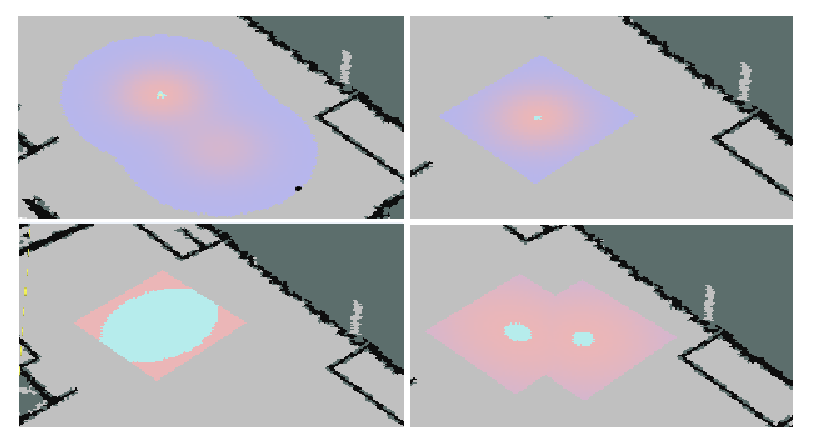
\includegraphics[width=0.42\textwidth]{pictures/all.eps}\label{fig:costmapPic}}%

\caption{Sample costmap shapes. Top right: standard 2D Gaussian, top left: Convolution method, bottom right: mean shift and bottom left: K-means.}
\label{fig:costmapPic}
\end{figure}

%1. FMM + without uncertainity\\2. FMM + with uncertainity\\	2a. Convolution\\	2b. clustering\\3. DWA + without uncertainity\\4. DWA + with uncertainity\\	2a. Convolution\\	2b. clustering\\

%All these should have simulations and real robot experiments.\\
\begin{figure}
%\left
\subfloat[]{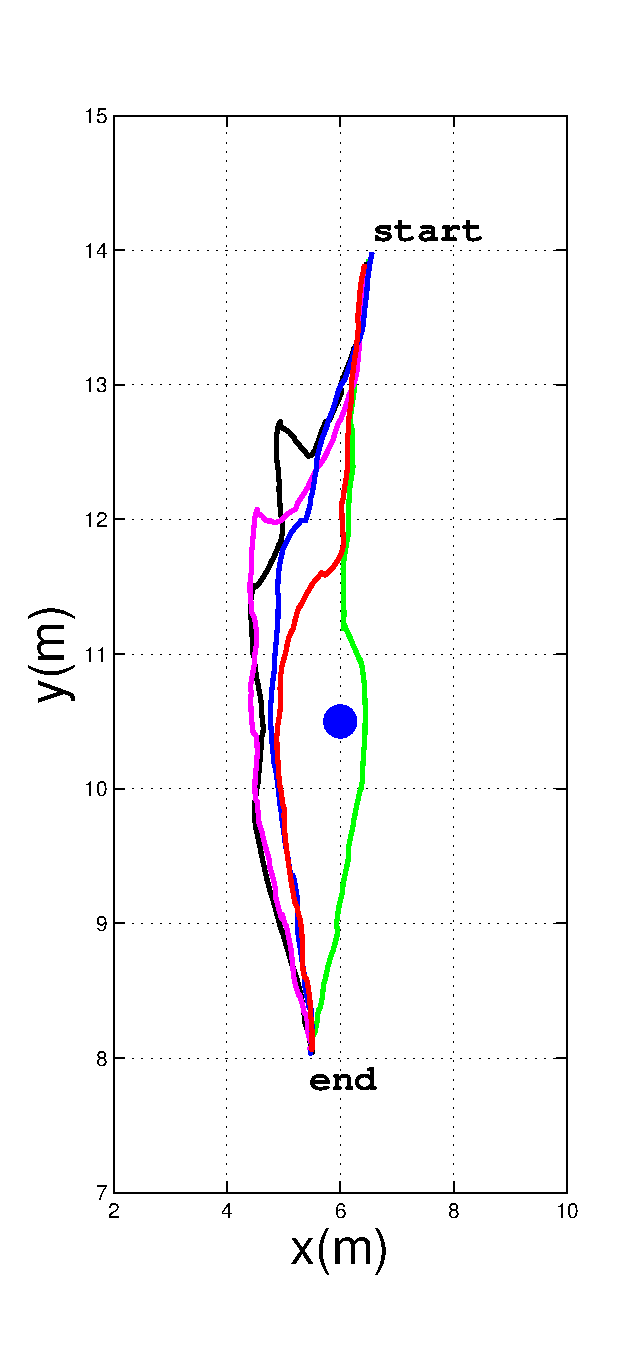
\includegraphics[width=0.17\textwidth, trim= 3mm 12.5mm 0mm 17.05mm, clip]{pictures/traj1.eps}\label{fig:traj1}}%
%\hspace{0.1cm}
\subfloat[]{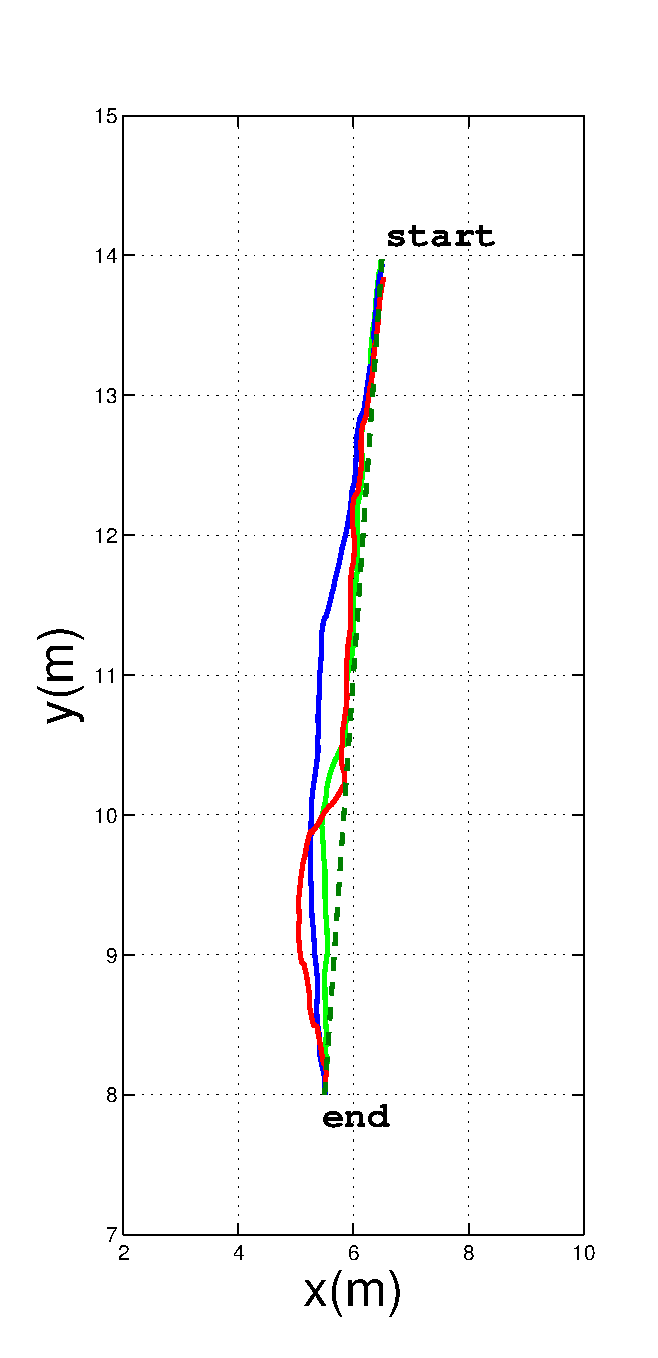
\includegraphics[width=0.17\textwidth, trim= 3mm 12.5mm 0mm 17.05mm, clip]{pictures/traj2.eps}\label{fig:traj2}}%
%\hspace{0.1cm}
\subfloat[]{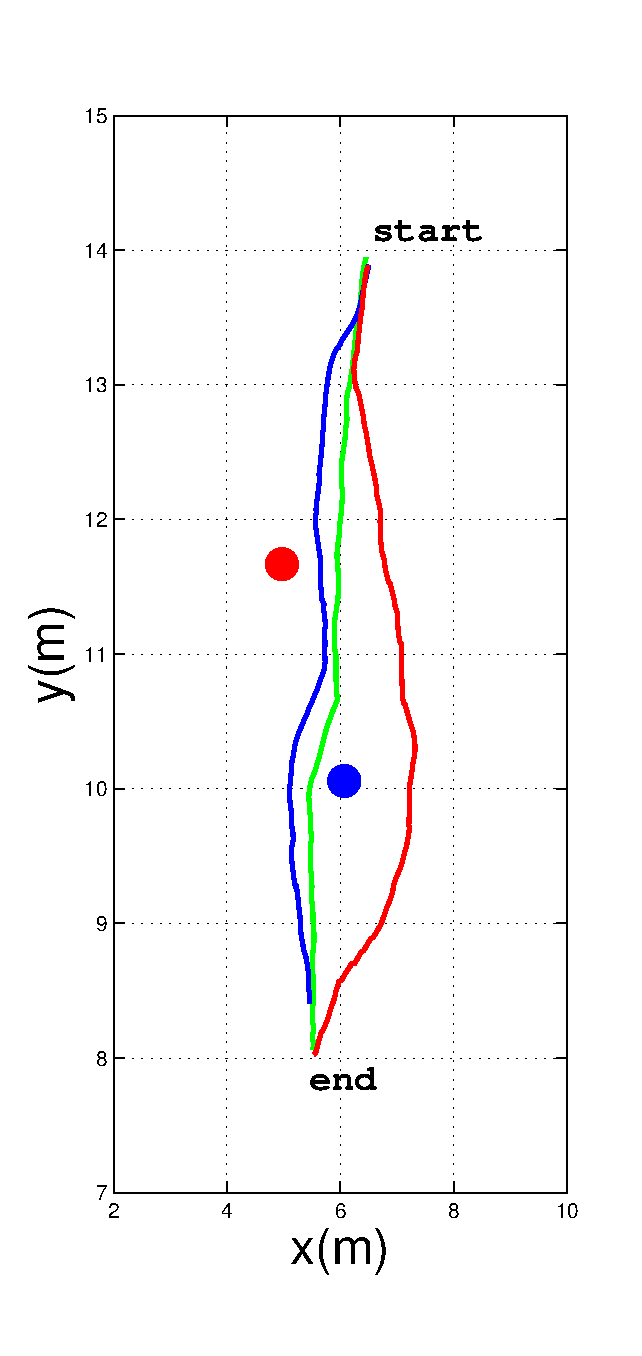
\includegraphics[width=0.17\textwidth, trim= 3mm 12.5mm 0mm 17.05mm, clip]{pictures/traj3.eps}\label{fig:traj3}}%
%\hspace{0.1cm}

\caption{Sample robot trajectories for different methods. Color coding: green for BN, red for DHA, black for KHA, pink for SHA and blue for CHA. Scenarios: (a) Single static person. (b) Single dynamic person. The person starts moving from the end point to the starting point of the robot's trajectory indicated by labels on the plots. (c) Two static people.
%Dots: static people.
}
\label{fig:trajs}
\end{figure}

\begin{figure*}
\centering
\subfloat[]{\includegraphics[width=0.170\textwidth, trim= 1mm 13mm 2mm 8mm, clip]{pictures/m1.eps}\label{fig:1_1}}%
%\hspace{%0.1cm}
\subfloat[]{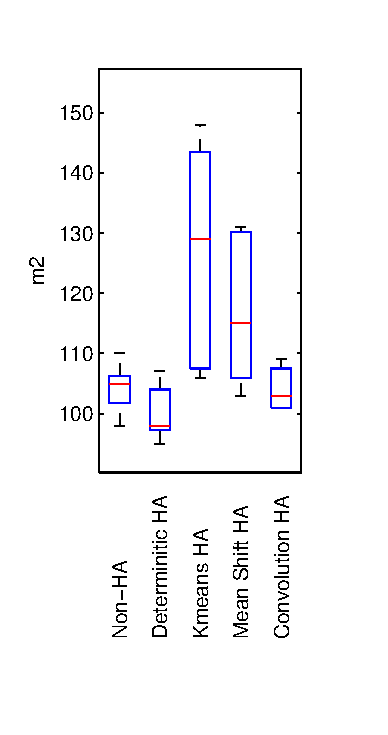
\includegraphics[width=0.170\textwidth, trim= 1mm 13mm 2mm 8mm, clip]{pictures/m2.eps}\label{fig:1_2}}%
%\hspace{0.1cm}
\subfloat[]{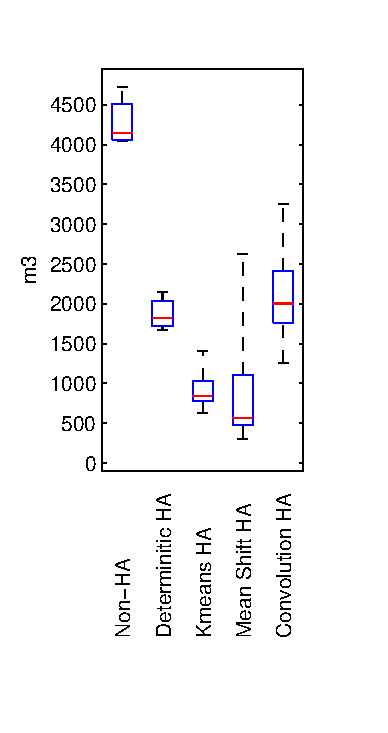
\includegraphics[width=0.170\textwidth, trim= 1mm 13mm 2mm 8mm, clip]{pictures/m3.eps}\label{fig:1_3}}%
%\hspace{0.1cm}
\subfloat[]{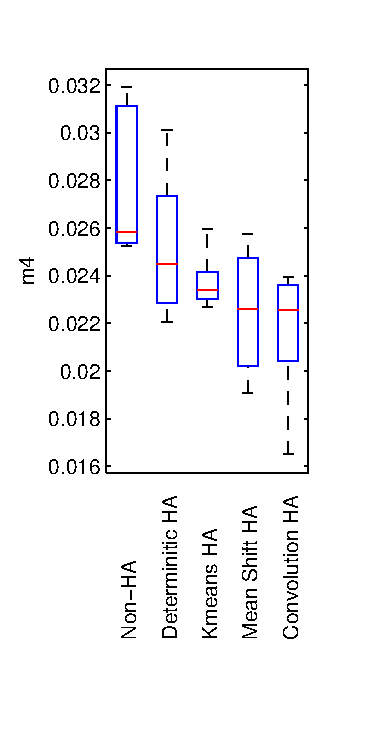
\includegraphics[width=0.170\textwidth, trim= 1mm 13mm 2mm 8mm, clip]{pictures/m4.eps}\label{fig:1_4}}%
%\hspace{0.1cm}
\subfloat[]{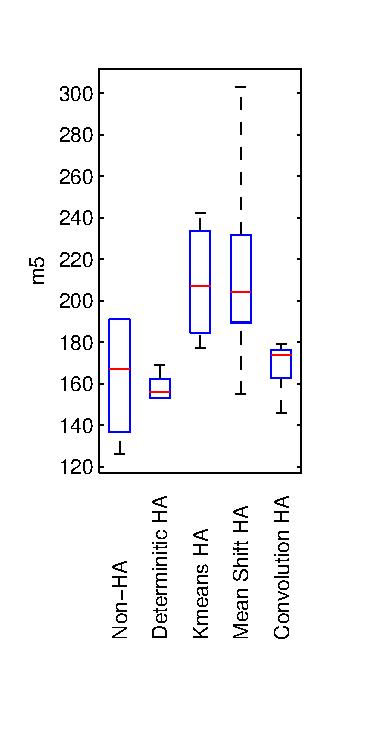
\includegraphics[width=0.17\textwidth, trim= 1mm 13mm 2mm 8mm, clip]{pictures/m5.eps}\label{fig:1_5}}%

\caption{Performance metrics obtained in the single static person scenario. HA stands for Human-Aware in the plot labels.
}
\label{fig:boxplots_singlePerson}
\end{figure*}

\subsection{Results}
\label{sec:results}
Figure \ref{fig:costmapPic} shows sample costmaps of the different methods mentioned earlier. It can be seen that the clustering methods can end up with saturated costs when the uncertainty is high due to large $\sigma$ values. The convolution costmap has a much more flexible shape and is not limited whereas other costmaps all have a cut off distance.

Sample trajectories of the robot are depicted in Fig. \ref{fig:trajs}. It is clear from the plots that HA methods result in trajectories that preserve larger distances to the people. Additionally, they are smoother and therefore more natural from the point of view of a person, this is supported by Fig. \ref{fig:1_4}, \ref{fig:2_2}, and \ref{fig:3_4}. However, this may not be evident from the trajectory plots. This is due to the abrupt movement of non-HA navigation upon encountering a person which considerably affects the smoothness. 

Clustering methods can cause the robot to modify its plan largely by enforcing a certain cluster shape upon finding cluster centroids: if the new probabilistic data leads to a new centroid that is not very close to the previous one, the costmap could change significantly and therefore the planned path. This is more severe for mean shift clustering due to adaptively modifying the number of clusters as well. This is to be expected given the probabilistic nature of the perception data, however the plan can be modified more smoothly using the convolution method. This method which outperforms all other methods in terms of smoothness in all of our tests, is shown to be a remedy to this problem based on our experimental results. Hence, for the second and third scenario, we only compare the results of 1) BN, 2) DHA, and 3) CHA methods.  

When comparing the results of DHA with CHA we can see that the former is a more conservative method in terms of keeping distance to the people when receiving accurate data. If DHA receives a perfect estimate of the person's position it can lead to the desired path, however this is seldom the case. Particularly, in the case of a moving person, the detector could not always keep up with the speed of the person, \textit{i.e.}, the position estimates were reported with delay or the person was lost in some cases, and the robot was faced with the human while considering him an obstacle. This led to abrupt changes and getting too close to the person, see Fig.~\ref{fig:traj2}. However, CHA by associating larger uncertainty to the estimates in this case, could lead to better plans in terms of proximity and smoothness. Unfortunately, due to our inaccurate ground truth of the moving person, we only rely on $m_{4}$ and $m_{5}$ for scenario 2, but we observed the delayed perception and lost person problem during our experiments. 




\begin{figure}[!]
\centering
\subfloat[]{\includegraphics[width=0.150\textwidth, trim= 0mm 13mm 2mm 8mm, clip]{pictures/dy_m4.eps}\label{fig:2_2}}%
\hspace{0.1cm}
\subfloat[]{\includegraphics[width=0.15\textwidth, trim= 0mm 13mm 2mm 8mm, clip]{pictures/dy_m5.eps}\label{fig:2_3}}%

\caption{Performance metrics obtained in the dynamic person scenario. %HA stands for Human-Aware in the plot labels.
}
\label{fig:boxplots_singlePersonMov}
\end{figure}

%
\begin{figure}[t!]
\centering
\subfloat[]{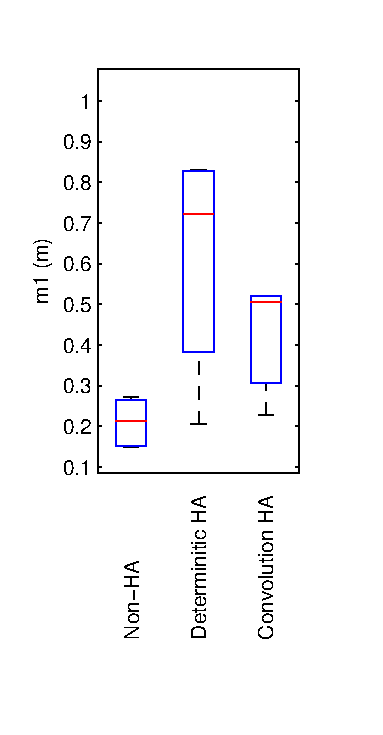
\includegraphics[width=0.163\textwidth, trim= 2mm 13mm 2mm 9mm, clip ]{pictures/two_m1.eps}\label{fig:3_1}}% \vspace{<whatever>}
%\hspace{0.1cm}
\subfloat[]{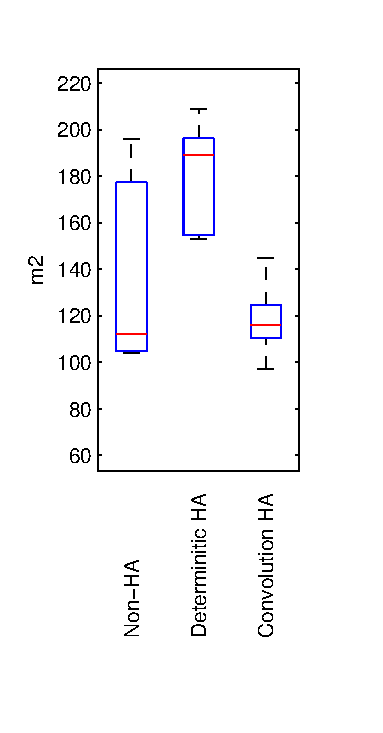
\includegraphics[width=0.163\textwidth, trim= 2mm 13mm 2mm 9mm, clip ]{pictures/two_m2.eps}\label{fig:3_2}}%
%\hspace{0.1cm}
\subfloat[]{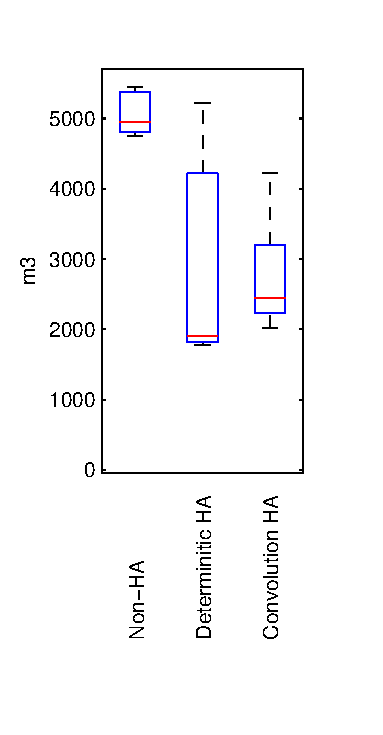
\includegraphics[width=0.163\textwidth, trim= 2mm 13mm 2mm 9mm, clip ]{pictures/two_m3.eps}\label{fig:3_3}}%

%\hspace{0.1cm}
\subfloat[]{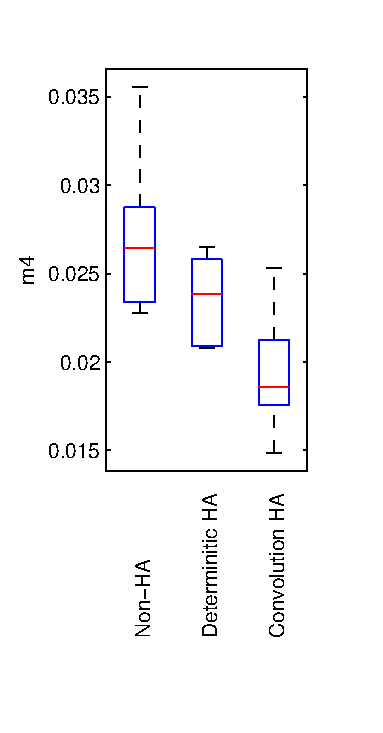
\includegraphics[width=0.163\textwidth, trim= 2mm 13mm 2mm 9mm, clip ]{pictures/two_m4.eps}\label{fig:3_4}}%
%\hspace{0.1cm}
\subfloat[]{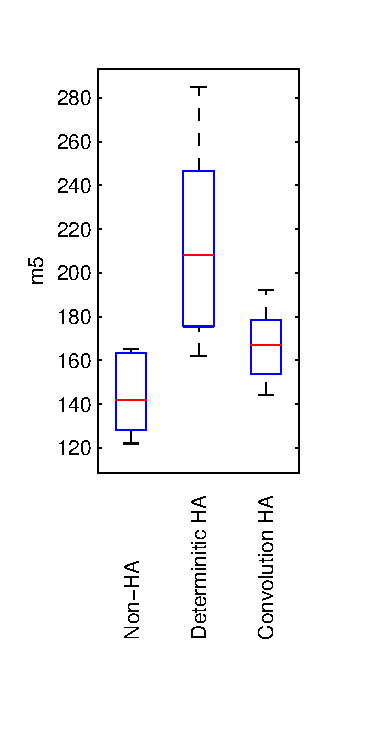
\includegraphics[width=0.163\textwidth, trim= 2mm 13mm 2mm 9mm, clip ]{pictures/two_m5.eps}\label{fig:3_5}}%
%\hspace{0.1cm}
%\subfloat[]{\includegraphics[width=0.163\textwidth, trim= 2mm 13mm 2mm 8mm, clip ]{pictures/two_m6.eps}\label{fig:3_6}}%

\caption{Performance metrics obtained in the two static people scenario.
% HA stands for Human-Aware in the plot labels.
}
\label{fig:boxplots_2people}
\end{figure}


Figures \ref{fig:boxplots_singlePerson}, \ref{fig:boxplots_singlePersonMov} and \ref{fig:boxplots_2people} show the performance metrics for the three scenarios. We will discuss the results of each metric in the following. $m_{1}$ has increased for HA methods which shows the effectiveness of our FMM planner in social path planning. However, DHA is more conservative in this regard in the presence of good perception data. $m_{2}$ has increased for uncertainty-based methods in the simple scenario as the deterministic tracker is giving already good position estimates, but this is no longer the case when the complexity is increased as seen in Fig. \ref{fig:3_2}. $m_{3}$ is also reduced for HA methods and more so for uncertainty-based HA methods as the complexity of the problem increases, see Fig.\ref {fig:3_3}.


$m_{4}$ is showing a very interesting result, we can see how uncertainty-based HA methods have managed to introduce smoothness into the trajectories by reducing jerk without deliberately accounting for it. CHA is dominating other methods across all scenarios in this case. Lastly, $m_{5}$ which shows the total navigation time is always lower for BN due to optimizing the path length only. The largest values belong to KHA and SHA due to constant modifications of the path, thus taking longer routes. For DHA this metric is lower than CHA for the static person case and comparable to CHA in the moving person scenario, but it increases as the complexity of the environment grows further in the case of multiple people.% Lastly, $m_{6}$ which is only used in the third scenario, indicates how DHA has varying behavior (sometimes takes a detour) based on the tracker estimates whereas CHA has more or less the same behavior in our runs due to its probabilistic nature when computing the social costmap.     



%\subsection{Discussion}
%\label{sec:discussion}

\section{Conclusion}
\label{sec:conclusion}

In this work we have proposed a novel approach for extending the model of social costmaps to include the uncertainty of perception. Experiments show how this extended model can lead to more natural robot trajectories that preserve a social distance from people. By combining the output of a probabilistic MCMC-based tracker with an expectation costmap computation method based on convolution, we introduce a principled approach to solve the social path planning problem in real environments with multiple people. 

The idea presented in this paper can be extended to other types of perception sources. By providing probabilistic perception outputs, the proposed model can fulfil this task without loss of performance. As future steps for this research, we plan to test other types of perception, particularly on-board perception which allows much more flexibility in terms of applications and fewer physical limitations. We also plan to incorporate orientation information and uncertainty of orientation in our model. Additionally, more tests with more accurate ground truth data can help to understand the problem and its challenges better. Moreover, quantifying the uncertainty of perception can be very useful in analyzing the behavior of expectation-based social costmap computation methods.  


\section*{Acknowledgements}

This work has been supported by the European MOnarCH project FP7-ICT-9-2011-601033. 
%\section{PROBABILISTIC TRACKING MODEL}
We are interested in the underlying \textit{state} of the environment which is modelled as a tuple: location and orientation of the people. The \textit{discriminative detectors} used to estimate these state variables have associated noise due to various state factors such as occlusion, lighting conditions, different posture of people, motion of the robot and the people. Coupled with this, there is also stochasitcity in the state transitions, which makes it hard to compute an exact estimate of the location of the people. A principled approach to solve this problem, is to compute a \textbf{belief} (posterior distribution) over the states using recursive bayesian estimation. More formally,

LeT $\textbf{X}_{t}$ be the state of the environment at time \textit{t}.
\begin{align}
P(\textbf{X}_{t} | \textbf{O}_{t}) = \dfrac{P(\textbf{O}_{t} | \textbf{X}_{t}) P(\textbf{X}_{t}|\textbf{X}_{t-1})} {P(\textbf{X}_{t-1})}
\end{align} 

Where, $P(\textbf{O}_{t} | \textbf{X}_{t})$ is the likelihood of the state given all our observations (detector outputs). Computation of this likelihood is best performed by using a learnt model of how the detectors perform for different states. Details of how these \textit{observation models} are created is explained in the next section.

$P(\textbf{X}_{t}|\textbf{X}_{t-1})$ is the \textit{transition model} which models the evolution of the state variables. For a multi person natural environment, an exact analyitical model is intractable. We model the motion of the people independently. we assume a first order model for motion incorporating velocity of the person. Interactions between people are environment specific and is outside the scope of this work. So we choose to ignore this aspect of the environment and attribute it to the uncertainity we have in the state estimation. The exact model for a multi person environment is given in section ......

Another important aspect is the computation of this belief itself. the state space is extremely complex so as to compute exactly this probability 
distribution over the states. We use an MCMC based sampling algorithm to approximately compute the belief. The details of our sampling alogorithm is given in section .......

%For the purpose of the human aware navigation planner, we transform these beliefs to a lower dimensional representation which is a 2-dimensional gaussian over the location of the person.

\subsection{Detector}
We use a probabilsitic background based detector
\subsection{Observation models}
We learn from data, the distribution $P(\textbf{O}|\textbf{X})$ for each detector. 




% \addtolength{\textheight}{-12cm}   % This command serves to balance the column lengths
                                  % on the last page of the document manually. It shortens
                                  % the textheight of the last page by a suitable amount.
                                  % This command does not take effect until the next page
                                  % so it should come on the page before the last. Make
                                  % sure that you do not shorten the textheight too much.

%%%%%%%%%%%%%%%%%%%%%%%%%%%%%%%%%%%%%%%%%%%%%%%%%%%%%%%%%%%%%%%%%%%%%%%%%%%%%%%%

% \section*{APPENDIX}
% Appendixes should appear before the acknowledgment.

%\section*{Acknowledgement}
%This research was supported by the Swiss National Science Foundation through the National Center of Competence in Research Robotics.
% The preferred spelling of the word �acknowledgment� in America is without an �e� after the �g�. Avoid the stilted expression, �One of us (R. B. G.) thanks . . .�  Instead, try �R. B. G. thanks�. Put sponsor acknowledgments in the unnumbered footnote on the first page.

%\begin{thebibliography}{99}
%\end{thebibliography}

%Equalize columns in last page
%\IEEEtriggeratref{11}


%\zt{Deepak I don't know what is wrong with the reference list}
\bibliographystyle{IEEEtran}
\bibliography{papers}

\end{document}
